\section{HarvestMem 方法}
\label{sec:method}

\subsection{总体框架与设计原则}
\label{sec:framework}
HarvestMem 的总体框架如图~\ref{fig:overview} 所示。它保留通用 VLA 的“视觉编码器 + VLM 骨干 + 记忆分支 + 动作专家”结构，在“\emph{记什么、怎么组织、事件从哪里来}”三个环节引入新设计：\pedet{}（创新一，第~\ref{sec:pedet} 节）回答\emph{何时发生了采摘}；\hem{}（创新二，第~\ref{sec:hem} 节）回答\emph{在固定预算下记住什么、如何编码}；事件鲁棒训练与事后确认自训练（创新三，第~\ref{sec:robust} 节）回答\emph{如何容忍检测误差、如何零标注落地真机}。设计遵循三条原则：

\textbf{P1：事件由物理定义，检测由学习完成。}“什么是一次采摘”由可测量的物理量定义（双指接触、果柄脱离），它在仿真中提供零成本的精确标签，在真机上可由作业结果事后确认；“如何从传感器流中识别它”交给学习型检测器。

\textbf{P2：按事件组织记忆，按时龄分层压缩。}近期事件保留完整细节以支持当下决策，远期事件只保留“在哪里摘过一颗”的摘要证据，场景锚与时间上下文各自占有固定位置。

\textbf{P3：不增加推理开销，可退化为基线。}记忆图像数、token 数和网络主体保持不变；新增嵌入零初始化，训练初始时与基础模型完全等价；当不发生事件时 \hem{} 自动退化为均匀记忆。

\subsection{数据链路与数据流}
\label{sec:dataflow}
图~\ref{fig:dataflow} 给出 HarvestMem 从数据生成到在线控制的完整链路，表~\ref{tab:dataflow} 列出其中流动的主要张量。

\begin{figure}[t]
\centering
\resizebox{\linewidth}{!}{%
\begin{tikzpicture}[font=\footnotesize, >=Stealth,
  nd/.style={draw=black!55, rounded corners=2pt, align=center, text width=2.3cm, minimum height=1.0cm, fill=black!4, font=\footnotesize},
  o1/.style={nd, draw=orange!80!black, thick, fill=orange!12},
  o2/.style={nd, draw=blue!70!black, thick, fill=blue!9},
  o3/.style={nd, draw=green!50!black, thick, fill=green!8},
  lab/.style={fill=white, inner sep=1pt, font=\scriptsize}]
\node[rotate=90, font=\footnotesize\bfseries] at (-0.45,3.55) {训练（离线）};
\node[rotate=90, font=\footnotesize\bfseries] at (-0.45,0.6) {部署（在线，20 Hz）};
\draw[black!25] (-0.2,2.4) -- (15.9,2.4);

\node[nd] (t1) at (1.3,3.2) {程序化场景生成\\{\scriptsize 果树·成熟度·遮挡·风}};
\node[nd] (t2) at (3.95,3.2) {专家示范采集\\{\scriptsize 干净 + DART-H 扰动}};
\node[o1] (t3) at (6.6,3.2) {物理自动标注\\{\scriptsize 接触·脱离·成败，零人工}};
\node[o3] (t4) at (9.25,3.2) {\Ciii{} 事件扰动 EPT\\{\scriptsize 漏检·误检·时间抖动}};
\node[o2] (t5) at (11.9,3.2) {\Cii{} HEM 构造记忆\\{\scriptsize $\{(m_i,\tau_i,\delta_i)\}_{i=1}^{16}$}};
\node[nd] (t6) at (14.55,3.2) {VLA 微调\\{\scriptsize 流匹配损失}};
\node[o1] (tp) at (9.25,4.55) {\Ci{} PEDet 训练\\{\scriptsize + 闭环回放·域随机化}};
\draw[->] (t1) -- (t2); \draw[->] (t2) -- (t3); \draw[->] (t3) -- (t4);
\draw[->] (t4) -- (t5); \draw[->] (t5) -- (t6);
\draw[->] (t3.north) |- (tp.west);

\node[nd] (d1) at (1.3,0.6) {传感器\\{\scriptsize $I^{f}_t,\ I^{w}_t,\ s_t$}};
\node[o1] (d2) at (3.95,0.6) {\Ci{} PEDet 逐帧推理\\{\scriptsize $p^{\mathrm c}_t,\ p^{\mathrm d}_t$}};
\node[o1] (d3) at (6.6,0.6) {迟滞解码\\{\scriptsize 事件表 $\mathcal E_t$}};
\node[o2] (d4) at (9.25,0.6) {\Cii{} HEM（每 16 步）\\{\scriptsize 分层选帧 + 拼图}};
\node[o2] (d5) at (11.9,0.6) {共享视觉编码\\{\scriptsize + 类型-时间嵌入}};
\node[nd] (d6) at (14.55,0.6) {VLA 推理\\{\scriptsize $A_t\in\mathbb R^{20\times8}$ $\rightarrow$ 安全包络 $\rightarrow$ 机械臂}};
\draw[->] (d1) -- (d2); \draw[->] (d2) -- (d3); \draw[->] (d3) -- (d4);
\draw[->] (d4) -- (d5); \draw[->] (d5) -- (d6);
\draw[->] (d1.south) -- ++(0,-0.4) -| node[lab, pos=0.25, below]{帧缓存：每帧 $4{\times}4$ 池化特征（基础结构已有）} ([xshift=-0.5cm]d4.south);
\draw[->, dashed, green!45!black, thick] ([xshift=-0.6cm]d6.north) -- ++(0,0.5) -| node[lab, pos=0.25, above=1pt]{\Ciii{} 事后确认自训练：作业结果 $\rightarrow$ 伪标签 $\rightarrow$ 更新 PEDet（无人工、无附加传感器）} (d2.north);
\draw[->, dashed, black!50] ([xshift=0.6cm]t6.south) -- node[lab, right]{权重} ([xshift=0.6cm]d6.north);
\end{tikzpicture}}
\caption{HarvestMem 的数据链路。上：离线训练链，仿真场景经专家示范、物理自动标注后分两路，一路训练 \pedet，另一路经事件扰动和 \hem{} 构造记忆，形成 VLA 训练样本 $(o_t,s_t,\ell,\mathcal M_t,A^\star_{t:t+20})$。下：在线控制流，\pedet{} 逐帧更新事件表，\hem{} 每次决策时从帧缓存中组织 16 幅记忆图像；回合结束后，作业结果用于事后确认伪标签。训练与部署使用同一个 \hem{} 构造函数。}
\label{fig:dataflow}
\end{figure}

\textbf{离线训练链。}(1) \emph{场景生成}：由布局种子程序化生成果树几何、果实位置与成熟度、遮挡叶片和风的时间表（第~\ref{sec:benchmark} 节）。(2) \emph{示范采集}：规范化专家与相位门控扰动专家（第~\ref{sec:platform} 节）在训练布局上采集示范，每帧记录前置与腕部图像、本体状态、动作标签，以及只用于标注的物理量（指尖接触对、果柄约束标志、果实位姿）。(3) \emph{物理自动标注}：按第~\ref{sec:event_def} 节的定义逐帧生成接触、脱离和成败标签，得到真值事件表 $\mathcal E^\star$。(4) \emph{检测器训练}：用示范和闭环回放训练 \pedet。(5) \emph{记忆构造}：对每个采样到的决策时刻 $t$，先以检测器的误差模型扰动 $\mathcal E^\star$，再由 \hem{} 构造 16 幅记忆图像及其类型和时龄，与当前观测和未来 20 步的专家动作组成训练样本。之所以不直接用 \pedet{} 在训练集上的输出，是因为检测器在自己的训练数据上几乎没有误差，无法反映部署时的真实误差分布（第~\ref{sec:ept} 节）。

\textbf{在线控制流。}每个控制步（20~Hz），前置与腕部图像、本体状态进入帧缓存，帧缓存按基础结构的做法保存每帧经视觉编码器池化后的 16 个 token；\pedet{} 同时对腕部图像和本体状态做一次推理并更新事件表。每 16 步进行一次决策：\hem{} 依据事件表从帧缓存中取出各层记忆帧的特征，摘要层的拼图帧仅在有事件进入摘要层时重新编码一次并缓存；记忆 token 叠加类型-时间嵌入后送入记忆分支，当前两路图像、指令和状态送入骨干，动作专家经 \V{fm_steps} 步流匹配积分输出 $20\times8$ 的动作块，执行前 16 步。回合结束后，事后确认模块根据夹爪与腕部相机记录的作业结果生成伪标签，周期性地更新 \pedet。

\begin{table}[t]
\centering
\caption{HarvestMem 数据流中的主要张量}
\label{tab:dataflow}
\small
\setlength{\tabcolsep}{4pt}
\begin{tabular}{llll}
\toprule
数据 & 形状 & 频率 & 去向\\
\midrule
前置/腕部图像 $I^{f}_t,I^{w}_t$ & $2\times256\times256\times3\rightarrow224\times224$ & 20~Hz & 视觉编码器，每路 256 token\\
腕部图像（检测用） & $128\times128\times3$ & 20~Hz & \pedet{} 视觉分支\\
本体状态 $s_t$ & 8（7 关节角 + 夹爪开度） & 20~Hz & 骨干（离散化 token）、\pedet\\
语言指令 $\ell$ & $\le 200$ token（与状态合计） & 每回合 & 骨干\\
事件概率 $p^{\mathrm c}_t,\,p^{\mathrm d}_t$ & 2 & 20~Hz & 迟滞解码\\
事件表 $\mathcal E_t$ & $\{(t^{\mathrm c}_e,t^{\mathrm d}_e)\}$ & 事件触发 & \hem\\
记忆图像 $\{m_i\}$ & $16\times224\times224\times3$（含拼图帧） & 每 16 步 & 共享视觉编码器\\
记忆 token & $16\times16\times2048$（$4\times4$ 池化） & 每 16 步 & 叠加类型-时间嵌入后进入记忆分支\\
动作块 $A_t$ & $20\times8$（7 关节增量 + 夹爪） & 每 16 步 & 安全包络 $\rightarrow$ 机械臂\\
\bottomrule
\end{tabular}
\end{table}

\subsection{基础策略结构}
\label{sec:base}
策略网络采用当前主流的“视觉-语言骨干 + 动作专家”结构\cite{black2024pi0,pi05_2025}，各部分均不作为本文贡献。当前的前置与腕部图像由冻结的 SigLIP 编码器\cite{zhai2023siglip}编码为每路 256 个 token，与指令和离散化的本体状态一起输入 Gemma-2B 视觉-语言骨干\cite{beyer2024paligemma}。历史记忆由一个约 150M 参数的记忆分支处理：每幅记忆图像经同一 SigLIP 编码后，把 $16\times16$ 的图像块特征平均池化为 $4\times4=16$ 个 token，叠加帧位置编码和该帧的本体状态嵌入；16 幅记忆图像共 256 个 token。约 300M 参数的动作专家以骨干和记忆分支的表示为条件，用流匹配\cite{lipman2023flow}生成 20 步动作块。模型从在通用操作数据上训练的检查点初始化，在 \bench{} 上微调全部非视觉参数。

\subsection{采摘事件的物理定义}
\label{sec:event_def}
一次\emph{采摘事件} $e=(t^{\mathrm c}_e,\,t^{\mathrm d}_e)$ 由两个物理时刻定义：
\begin{itemize}
\item \textbf{接触} $t^{\mathrm c}_e$：夹爪闭合过程中两指首次同时与同一颗果实接触，并持续至少 2 个控制步；
\item \textbf{脱离} $t^{\mathrm d}_e$：该果实的果柄约束解除、且果实仍被夹持的第一个控制步。
\end{itemize}
只有接触之后在时间窗 $T_{\max}$ 内发生脱离，才构成一次\emph{成功采摘}；接触后未脱离（抓空、滑脱、拉拽失败）记为\emph{失败尝试}。该定义不涉及成熟度：摘下青果同样是一次采摘事件，是否该摘是策略的决策问题，而不是记忆组织的问题，这避免了把成熟度真值通过记忆间接泄露给策略。仿真中两个时刻都可从物理状态直接读出，因此标签自动、精确且零成本。作为对照，文献中常用的\emph{几何事件}以 TCP 到最近仍挂树果实的距离
\begin{equation}
d_t=\min_{j\in\mathcal P_t}\lVert p^{\mathrm{TCP}}_t-c_j\rVert_2
\label{eq:signal}
\end{equation}
定义：$d_t\le r$ 的最长连续段构成一个事件（$r=\V{radius_r}$~cm，$\mathrm{tol}=\V{tol}$~mm）。几何事件需要果实位置真值，而且会把每一次失败尝试都记为一次“采摘”。

\subsection{创新一：物理监督的学习型采摘事件检测器 \pedet}
\label{sec:pedet}
\pedet{} 要在不使用任何特权信息的条件下，从机器人自身的传感器流中因果地给出\emph{成功}采摘事件。其结构如图~\ref{fig:pedet} 所示。

\begin{figure}[t]
\centering
\resizebox{\linewidth}{!}{%
\begin{tikzpicture}[font=\footnotesize,
  blk/.style={draw, rounded corners=2pt, align=center, minimum height=0.8cm, inner sep=3pt, fill=white},
  arr/.style={-{Stealth[length=1.8mm]}, thick}]
\node[blk, fill=gray!8] (img) {腕部 RGB\\$128\times128$};
\node[blk, fill=gray!8, below=0.55cm of img] (prop) {本体特征\\$q_t$, $w_t$, $u_t$, $\Delta w_t$};
\node[blk, right=0.5cm of img, fill=blue!6] (cnn) {ResNet-18\\（ImageNet 初始化）};
\node[blk, right=0.5cm of prop, fill=blue!6, minimum width=2.15cm] (mlp) {MLP\\$2\times 64$};
\node[blk, right=0.5cm of cnn, yshift=-0.68cm, fill=blue!6] (fuse) {拼接\\$128+64$};
\node[blk, right=0.5cm of fuse, fill=orange!12, minimum width=2.2cm] (tcn) {因果时序卷积\\4 层，膨胀 1/2/4/8\\感受野 31 帧};
\node[blk, right=0.6cm of tcn, yshift=0.9cm, fill=red!6] (hc) {接触头 $p^{\mathrm c}_t$};
\node[blk, right=0.6cm of tcn, fill=red!6] (hd) {脱离头 $p^{\mathrm d}_t$};
\node[blk, right=0.6cm of tcn, yshift=-0.9cm, fill=gray!6] (hr) {距离头 $\hat d_t$（辅助）};
\node[blk, right=0.5cm of hd, fill=green!6] (dec) {迟滞解码\\成功采摘 $e$\\$(t^{\mathrm c},t^{\mathrm d})$};
\draw[arr] (img) -- (cnn); \draw[arr] (prop) -- (mlp);
\draw[arr] (cnn.east) -- ++(0.2,0) |- (fuse.west);
\draw[arr] (mlp.east) -- ++(0.2,0) |- (fuse.west);
\draw[arr] (fuse) -- (tcn);
\draw[arr] (tcn.east) -- ++(0.25,0) |- (hc.west);
\draw[arr] (tcn) -- (hd);
\draw[arr] (tcn.east) -- ++(0.25,0) |- (hr.west);
\draw[arr] (hc.east) -- ++(0.15,0) |- ([yshift=0.15cm]dec.west);
\draw[arr] (hd) -- (dec);
\node[below=0.25cm of mlp, align=center, text=green!40!black, xshift=1.9cm] {监督信号——仿真：物理状态自动生成；真机：作业结果事后确认（第~\ref{sec:hsl} 节）。两者均无需人工标注};
\end{tikzpicture}}
\caption{\pedet{} 结构。$q_t$ 为关节角，$w_t$ 为夹爪开度，$u_t$ 为夹爪指令，$\Delta w_t$ 为开度变化率。时序卷积只使用当前及过去的帧，检测是因果的。}
\label{fig:pedet}
\end{figure}

\textbf{多模态因果结构。}选择腕部相机，是因为接触和脱离在腕部视角中最清晰，且不受前方叶片遮挡；本体感知则提供与光照无关的“夹住了东西”的证据，两者互补。图像经 ResNet-18\cite{he2016resnet}编码并投影到 128 维，本体特征经两层 MLP 编码为 64 维，拼接后送入 4 层因果时序卷积网络\cite{bai2018tcn,lea2017tcn}（膨胀系数 1、2、4、8，感受野 31 帧，约 1.5~s）。网络有三个输出头：接触概率 $p^{\mathrm c}_t$、脱离概率 $p^{\mathrm d}_t$ 以及截断到 15~cm 的距离估计 $\hat d_t$；距离头只作为辅助任务帮助网络学习“靠近”的几何结构，不参与解码。

\textbf{物理监督与困难负样本。}由第~\ref{sec:event_def} 节的定义，$y^{\mathrm c}_t=1$ 当且仅当两指正与同一果实接触；脱离标签在 $t^{\mathrm d}_e$ 处取 1 并以 $\sigma=1$ 帧的高斯核平滑，以容忍一帧的时间误差；失败尝试的所有帧脱离标签均为 0。训练数据除专家示范外，还加入基础策略在训练布局上的闭环回放，其中大量的抓空、滑脱和重试构成了区分成功与失败所需的\emph{困难负样本}，这是几何定义和手工感知链路都无法提供的。损失函数为
\begin{equation}
\mathcal L_{\mathrm{det}}=\mathcal L_{\mathrm{focal}}(p^{\mathrm c},y^{\mathrm c})+\lambda_{\mathrm d}\,\mathcal L_{\mathrm{focal}}(p^{\mathrm d},\tilde y^{\mathrm d})+\lambda_{\mathrm r}\,\mathbb 1[d_t<0.15]\,\mathrm{SmoothL1}(\hat d_t,d_t),
\end{equation}
其中 focal 损失\cite{lin2017focal}缓解事件帧极度稀少带来的类别不平衡，$\lambda_{\mathrm d}=2$，$\lambda_{\mathrm r}=0.5$。训练时施加域随机化\cite{tobin2017domain}：亮度增益 0.5--1.6、色温偏移、叶片与背景纹理替换、果实色调抖动、腕部相机位姿扰动（$\pm2$~cm、$\pm3^\circ$）、噪声、运动模糊和 JPEG 压缩。

\textbf{因果迟滞解码。}对 $p^{\mathrm c}_t$ 使用迟滞阈值：超过 0.6 进入接触段，低于 0.4 才退出，短于 3 帧的段被丢弃。接触关键帧取接触段开始后 5 帧内 $p^{\mathrm c}_t$ 最大的帧，即夹爪包稳果实的时刻；若接触段内或结束后 5 帧内 $p^{\mathrm d}_t$ 出现超过 0.5 的峰值，以峰值帧为脱离关键帧，确认一次成功采摘；否则记为失败尝试，不进入事件表。进行中的接触段只提供暂定接触帧，保证因果性。

\subsection{创新二：事件中心分层记忆 \hem}
\label{sec:hem}
第~\ref{sec:coverage} 节表明，均匀记忆记得住的采摘次数是一个与作业量无关的常数，而平坦事件关键帧的容量受“每次采摘占两帧”所限。\hem{} 的核心思想是：\textbf{近期事件保细节，远期事件保证据，场景与时间各有其位}。它把 $B$ 个记忆位置组织为四层（图~\ref{fig:hem}）：
\begin{equation}
B=|\mathcal A_t|+|\mathcal W_t|+|\mathcal S_t|+|\mathcal U_t|.
\end{equation}

\begin{figure}[t]
\centering
\resizebox{\linewidth}{!}{%
\begin{tikzpicture}[font=\scriptsize, >=Stealth,
  slot/.style={draw=black!60, minimum width=0.85cm, minimum height=0.85cm, inner sep=0pt},
  sA/.style={slot, fill=teal!25}, sW/.style={slot, fill=orange!35}, sS/.style={slot, fill=blue!18}, sU/.style={slot, fill=black!7}]
\draw[->, thick, black!60] (0,2.6) -- (14.9,2.6) node[right]{$t$};
\node[diamond, draw=teal!70!black, fill=teal!25, inner sep=1.4pt] at (0.25,2.6) {};
\node[above] at (0.25,2.72) {锚};
\foreach \i in {1,...,10} {
  \pgfmathsetmacro{\x}{1.2+(\i-1)*1.38}
  \ifnum\i<9
    \node[circle, draw=blue!70!black, fill=blue!18, inner sep=1.6pt] at (\x,2.6) {};
  \else
    \node[circle, draw=orange!80!black, fill=orange!35, inner sep=1.6pt] at (\x,2.6) {};
  \fi
  \node[above] at (\x,2.72) {$e_{\i}$};
}
\draw[decorate, decoration={brace, mirror, amplitude=4pt}] (1.0,2.4) -- (5.55,2.4) node[midway, below=4pt] (b1) {拼图帧 $S_1$};
\draw[decorate, decoration={brace, mirror, amplitude=4pt}] (6.5,2.4) -- (11.07,2.4) node[midway, below=4pt] (b2) {拼图帧 $S_2$};
\draw[decorate, decoration={brace, mirror, amplitude=4pt}] (12.0,2.4) -- (13.8,2.4) node[midway, below=4pt] (b3) {工作层 $\mathcal W$};

\foreach \j/\sty/\txt in {0/sA/{$I_0$}, 1/sS/{}, 2/sS/{}, 3/sW/{$c_9$}, 4/sW/{$d_9$}, 5/sW/{$c_{10}$}, 6/sW/{$d_{10}$}} {
  \node[\sty] (s\j) at (\j*0.93+0.425,0.6) {\txt};
}
\foreach \j in {7,...,15} { \node[sU] (s\j) at (\j*0.93+0.425,0.6) {$u$}; }
\foreach \j/\a/\b/\c/\d in {1/1/2/3/4, 2/5/6/7/8} {
  \draw[black!50] (s\j.north) -- (s\j.south); \draw[black!50] (s\j.west) -- (s\j.east);
  \node[font=\tiny] at ([xshift=-0.21cm, yshift=0.21cm]s\j.center) {\a};
  \node[font=\tiny] at ([xshift=0.21cm, yshift=0.21cm]s\j.center) {\b};
  \node[font=\tiny] at ([xshift=-0.21cm, yshift=-0.21cm]s\j.center) {\c};
  \node[font=\tiny] at ([xshift=0.21cm, yshift=-0.21cm]s\j.center) {\d};
}
\draw[->, black!50] (b1.south) -- (s1.north);
\draw[->, black!50] (b2.south) -- (s2.north);
\draw[->, black!50] (b3.south) -- ([xshift=0.45cm]s4.north);
\draw[->, black!50] (0.25,2.45) -- (s0.north);
\draw[decorate, decoration={brace, mirror, amplitude=4pt}] ([yshift=-0.08cm]s7.south west) -- ([yshift=-0.08cm]s15.south east) node[midway, below=4pt] {时间上下文层 $\mathcal U$：其余帧中等距选取（含失败尝试、场景演变）};
\node[anchor=north west, align=left] at (-0.05,-0.7) {\sq{teal!70!black} 场景锚 $\mathcal A$\quad \sq{blue!70!black} 情景摘要 $\mathcal S$（每格 $112^2$，对齐 $2\times2$ token）\\ \sq{orange!80!black} 工作事件 $\mathcal W$（接触 $c$ / 脱离 $d$）\quad \sq{black!40} 时间上下文 $\mathcal U$};
\end{tikzpicture}}
\caption{\hem{} 的记忆布局示例（第 10 次采摘之后的决策时刻，$B=16$）。最近 2 次采摘保留完整的接触帧与脱离帧；更早的 8 次采摘被压缩进 2 幅事件拼图帧，每格是一次采摘脱离后以 TCP 为中心的局部图像；第 0 帧作为场景锚；其余 9 个位置按时间等距选取。同样的 16 个位置，均匀记忆平均只能覆盖约 \V{cap_u} 次采摘，平坦关键帧（$k=8$）只能覆盖 4 次。}
\label{fig:hem}
\end{figure}

\textbf{场景锚层 $\mathcal A_t$。}包含第 0 帧以及最近一次场景切换（如换到下一株植物）后的第一帧，最多 2 个位置。场景切换时刻由平台的移动信号给出，不需要视觉检测。这一层承载场景记忆：叶片被风吹动之前看到的成熟果实。

\textbf{工作事件层 $\mathcal W_t$。}最近 $m_w=\V{hem_mw}$ 次成功采摘的接触帧与脱离帧，以完整分辨率保留“刚刚做了什么”的细节，支持避免重复抓取同一颗果、确认刚才的放果等即时决策。

\textbf{情景摘要层 $\mathcal S_t$ 与事件拼图帧。}更早的采摘按时间分组，每 $c=\V{hem_c}$ 次合成一幅\emph{事件拼图帧}，最多 $s_{\max}=\V{hem_smax}$ 幅。对事件 $e$，取其脱离后第 3 帧的前置图像，以 TCP 的图像投影为中心裁出局部区域并缩放到 $112\times112$，作为“在这里摘下过一颗果”的证据；4 个局部图像按时间顺序拼为一幅 $224\times224$ 图像，空格以中性灰填充并在注意力中屏蔽。拼图帧有一个关键的结构性质：SigLIP 把 $224\times224$ 图像切成 $16\times16$ 个图像块，记忆分支再平均池化为 $4\times4$ 个 token，因此每个 $112\times112$ 格恰好对应 $8\times8$ 个图像块、池化后的 $2\times2$ 个 token，\textbf{格与格之间在池化时互不混叠}。于是拼图帧在不增加 token、不引入新编码器的前提下，把 4 次采摘的证据装进一个记忆位置。远期事件只需回答“是否摘过、在哪里摘过”，不需要操作细节，较低的分辨率足以满足需要。

\textbf{时间上下文层 $\mathcal U_t$。}其余位置在不属于前三层的帧中等距选取，保留场景演变、失败尝试和回合进度的连续信息。

\textbf{自适应预算分配。}各层的位置数随事件数 $n$ 自动调整：
\begin{equation}
|\mathcal W_t|=2\min(n,m_w),\qquad |\mathcal S_t|=\Big\lceil \frac{\min\big(\max(n-m_w,0),\ c\,s_{\max}\big)}{c}\Big\rceil,\qquad |\mathcal U_t|=B-|\mathcal A_t|-|\mathcal W_t|-|\mathcal S_t|.
\end{equation}
回合初期尚无事件时，几乎全部位置用于时间上下文，\hem{} 退化为均匀记忆；事件累积后，事件层至多占用 $2m_w+s_{\max}=7$ 个位置，时间上下文始终保留至少 7 个位置。构造过程见算法~\ref{alg:hem}。

\begin{algorithm}[t]
\caption{\hem{} 在决策时刻 $t$ 的记忆构造}
\label{alg:hem}
\small
\begin{algorithmic}[1]
\Require 帧缓存 $I_{0:t}$，成功采摘事件表 $\mathcal E_t=(e_1,\dots,e_n)$，场景切换时刻 $t^{\mathrm s}$，预算 $B$，参数 $m_w,c,s_{\max}$
\Ensure 记忆 $\mathcal M_t=\{(m_i,\tau_i,\delta_i)\}_{i=1}^{B}$
\If{$t+1\le B$} \Return $\{(I_f,\textsc{上下文},t-f)\}_{f=0}^{t}$ \EndIf
\State $\mathcal A\gets\{0,\ t^{\mathrm s}\}$ \Comment{场景锚}
\State $\mathcal W\gets\{(t^{\mathrm c}_e,\textsc{接触}),\ (t^{\mathrm d}_e,\textsc{脱离}):\ e\in(e_{n-m_w+1},\dots,e_n)\}$ \Comment{工作事件层}
\State $\mathcal O\gets(e_{\max(1,\,n-m_w-c\,s_{\max}+1)},\dots,e_{n-m_w})$ \Comment{进入摘要层的事件}
\For{$\mathcal O$ 中按时间顺序每 $c$ 个事件组成的组 $g$}
  \State $m_g\gets\textsc{Mosaic}\big(\{\textsc{Crop}(I^{f}_{t^{\mathrm d}_e+3},\ \mathrm{TCP}_{t^{\mathrm d}_e+3}):e\in g\}\big)$，加入 $\mathcal S$ \Comment{事件拼图帧}
\EndFor
\State $n_U\gets B-|\mathcal A|-|\mathcal W|-|\mathcal S|$；$R\gets\{0,\dots,t\}\setminus(\mathcal A\cup\mathcal W)$
\State $\mathcal U\gets\{R[\lfloor i(|R|-1)/(n_U-1)\rfloor]:\ i=0,\dots,n_U-1\}$ \Comment{时间上下文层}
\State \Return $\mathcal A\cup\mathcal W\cup\mathcal S\cup\mathcal U$ 按时间排序，附类型 $\tau$ 与时龄 $\delta=t-f$
\end{algorithmic}
\end{algorithm}

\textbf{类型-时间嵌入。}分层之后，同一个记忆位置上可能是场景锚、接触瞬间、脱离瞬间、拼图帧或普通上下文帧，策略需要知道每幅记忆“是什么、多久以前”。基础结构中的帧位置编码只表示排列顺序，无法表达这些信息。为此，对记忆图像 $i$ 的第 $j$ 个 token，在视觉特征 $h_{i,j}$ 上叠加
\begin{equation}
z_{i,j}=h_{i,j}+\mathbf e_{\tau_{i,j}}+g\big(\phi(\delta_{i,j})\big),\qquad \tau\in\{\text{锚},\text{接触},\text{脱离},\text{摘要},\text{上下文}\},
\end{equation}
其中 $\mathbf e_\tau\in\mathbb R^{2048}$ 为可学习的类型嵌入，$\phi(\delta)$ 是 $\log(1+\delta)$ 的 16 频正弦特征，$g$ 为 $32\rightarrow64\rightarrow2048$ 的两层 MLP。对拼图帧，每个格对应的 $2\times2$ 个 token 各自使用该格事件的时龄，因此一幅拼图帧内的 4 次采摘仍可区分先后。类型嵌入和 $g$ 的最后一层均\emph{零初始化}，训练开始时模型与基础模型完全等价，新增参数仅约 \V{hem_params}~M。

\textbf{性质。}\hem{} 具有以下性质。\emph{预算与开销不变}：恒输出 $B$ 幅记忆图像、$16B$ 个 token；拼图帧只在有事件进入摘要层时编码一次，构造耗时约 \V{hem_ms}~ms。\emph{严格包含基线}：$m_w=s_{\max}=0$ 时即均匀记忆，$s_{\max}=0$ 时即平坦事件关键帧。\emph{因果且训练部署一致}：只使用已确认的事件，训练样本与在线决策调用同一构造函数。其事件容量由下述命题给出。

\begin{proposition}[分层记忆的事件容量]
\label{prop:capacity}
若事件检测正确，则在任意决策时刻，\hem{} 保留最近 $\min(n,\ m_w+c\,s_{\max})$ 次采摘的直接证据，至多占用 $2m_w+s_{\max}$ 个事件位置；占用同样多位置的平坦事件关键帧至多保留 $\lfloor(2m_w+s_{\max})/2\rfloor$ 次。
\end{proposition}
\noindent 取 $B=16$、$m_w=2$、$c=4$、$s_{\max}=3$，\hem{} 用 7 个事件位置保留 \V{cap_hem} 次采摘，平坦方案用 8 个位置只保留 4 次，且容量可通过 $c$ 和 $s_{\max}$ 继续扩展。图~\ref{fig:capacity} 在合成事件序列上验证了这一点：均匀记忆平均只覆盖约 \V{cap_u} 次采摘，平坦关键帧在第 4 次之后饱和于约 \V{cap_k8} 次，\hem{} 在 14 次以内全部覆盖。

\begin{figure}[t]
\centering
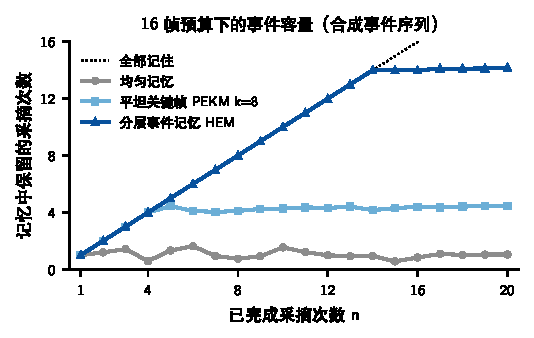
\includegraphics[width=0.62\linewidth]{zh_capacity}
\caption{16 帧记忆预算下保留的采摘次数（真实计算）。合成事件序列中相邻采摘间隔服从 $U(110,190)$ 帧，每个 $n$ 重复 300 次；某次采摘被计为保留，当且仅当记忆中有一帧落在其接触或脱离帧 $\pm3$ 帧内，或该采摘位于拼图帧中。}
\label{fig:capacity}
\end{figure}

\subsection{创新三：事件鲁棒训练与免标注真机适配}
\label{sec:robust}

\subsubsection{事件扰动训练（EPT）}
\label{sec:ept}
训练时若直接使用物理真值事件，策略看到的记忆永远“完美”，会学会无条件信任记忆；而部署时 \pedet{} 不可避免地存在少量漏检、误检和时间偏差，例如漏掉一次脱离会让记忆中少一次采摘，诱发多摘。我们提出\emph{事件扰动训练}：以概率 $\rho=0.5$ 对每个训练样本的真值事件表 $\mathcal E^\star$ 施加扰动 $\tilde{\mathcal E}=\Pi(\mathcal E^\star)$，包括 (1) 以概率 $p_{\mathrm{miss}}$ 删除事件；(2) 以概率 $p_{\mathrm{fp}}$ 把失败尝试误标为成功采摘，若该回合无失败尝试，则在接近阶段随机插入；(3) 把每个关键帧在 $\{-2,\dots,2\}$ 帧内随机偏移。扰动率按检测器在真机上的误差水平设定（$p_{\mathrm{miss}}=p_{\mathrm{fp}}=0.05$），比仿真误差更保守。被删除的事件仍可能出现在时间上下文层中，于是策略学会把事件层与上下文层、当前观测相互印证，而不是盲信任何单一来源。

\subsubsection{事后确认自训练（HSL）}
\label{sec:hsl}
真机上没有仿真物理状态，人工逐帧标注接触与脱离又费时费力；在果实或植株上加装传感器在生产中也不可行。我们的关键观察是：\textbf{一次采摘是否成功，在发生的瞬间难以判断，但在事后很容易确认}——成功的采摘必然以“夹着果实到达集果篮并松开”结束。据此提出\emph{事后确认自训练}，只使用夹爪开度、腕部相机和标定一次的篮区位置：
\begin{enumerate}
\item \textbf{持物段提取。}夹爪闭合指令发出后，若开度在 5 帧以上停滞在果实尺寸对应的区间内，即判定夹爪中有物体，记为一个持物段 $[t_a,t_b]$。
\item \textbf{结果确认。}若段末夹爪在篮区上方张开，且腕部图像中两指之间区域由“有果”变为“空”（与张开前相比的像素差超过阈值），确认为\emph{成功}；若开度在到达篮区之前塌缩到全闭（滑脱），或在篮区外张开，确认为\emph{失败}；闭合后开度直接到底的抓空同样记为失败。
\item \textbf{时刻回溯。}成功段的接触帧取持物段起点，脱离帧取段内当前 \pedet{} 的 $p^{\mathrm d}_t$ 最大值；若机械臂提供关节电流，拉拽时的电流峰值可作为辅助证据。失败段内所有帧的脱离标签为 0，构成纠正误检的困难负样本。
\item \textbf{一致性筛选与迭代。}只保留脱离帧位于拉拽阶段（TCP 离开接触位置 5~cm 之前）且 $\max p^{\mathrm d}_t>0.3$ 的成功段；用伪标签与仿真数据混合微调 \pedet{}（冻结视觉骨干前三个阶段），再用更新后的检测器重新回溯脱离帧，共迭代 2 轮。
\end{enumerate}
HSL 不需要任何人工标注，也不需要在果实、果柄或植株上加装传感器，可以在日常作业中持续运行，使检测器随作物、季节和光照的变化自我更新。在真机实验中，\pct{hsl_keep} 的持物段通过一致性筛选，伪标签相对人工标注的事件精确率为 \V{hsl_prec}（第~\ref{sec:res_real} 节）。

\subsection{低层执行平台}
\label{sec:platform}
\label{sec:dart}
记忆方法能否在闭环中体现价值，取决于低层执行是否可靠。早期实验中，策略常在搬运和放果后出现腕关节大幅偏转、长时间停滞等问题，成败主要由操作失误决定。为此，我们对执行平台做了四项改进并在训练前冻结：(1) \emph{规范化专家}：基于 mplib\cite{mplib}的脚本专家以固定休息位姿作为逆运动学初值，分区设置碰撞裕度并加入收臂路点，消除示范中的多峰腕部姿态；(2) \emph{相位门控恢复示范（DART-H）}：参照 DART\cite{laskey2017dart}，只在接近、搬运等自由运动阶段注入 Ornstein--Uhlenbeck 关节噪声（$\sigma=0.04$~rad，$\tau=10$ 步），记录从扰动状态重新规划的干净动作作为标签，以缓解协变量偏移\cite{ross2011dagger}；(3) \emph{观察期保持}：回合前 30 步机械臂静止，这些帧只作为历史进入记忆；(4) \emph{安全包络}：把关节目标裁剪到示范分布的 [0.5\%, 99.5\%] 分位区间外扩 0.1~rad，并限制单步增量。在 dev 布局上，这些改进使均匀记忆策略的整任务成功率从 \pct{ll_succ_a} 提高到 \pct{ll_succ_b}，首颗果实入篮率从 \pct{ll_first_a} 提高到 \pct{ll_first_b}，腕部失控率从 \pct{ll_wrist_a} 降到 \pct{ll_wrist_b}，放果后恢复运动的中位步数从 \V{ll_resume_a} 降到 \V{ll_resume_b}。所有记忆条件共用同一平台。
